\documentclass{article}
\usepackage{amsmath, amssymb}
\usepackage{cancel}
\usepackage{tikz}
\usepackage{tikz-cd}
\usepackage{mdframed}
\usepackage{hyperref}
\usetikzlibrary{automata, positioning, arrows}

\begin{document}

\section{Lecture 17: Plan for Class}
Last time:
\begin{enumerate}
    \item Smale horseshoe where the initial set is 
    \begin{enumerate}
        \item a Cantor set
        \item measure zero 
        \item uncountable $\infty$ 
    \end{enumerate}
    \item The dynamics of the Smale horseshoe are the same as a shift on two symbols 
\end{enumerate}

Today:
\begin{enumerate}
    \item Chain recurrence \S 5.2
    \item Hyperbolic structure \S 5.2
    \item Stable manifold theorem for hyperbolic sets \S 5.2
    \item $\Lambda$ lemma \S 5.2
    \item Markov partitions \S 5.3
    \item Subshift of finite type \S 5.3
    \item Sketch proof of Smale-Birkhoff theorem \S 5.3
\end{enumerate}

\section{Recurrence}

We have a few different objects in recurrence
\begin{itemize}
    \item fixed point 
    \begin{itemize}
        \item You approach some point asymptotically 
    \end{itemize}
    \item periodic orbit 
    \begin{itemize}
        \item You follow some cycle upon further applications of recurrence
    \end{itemize}
    \item nonwandering point 
    \begin{itemize}
        \item If you start at some point, you will return to a neighborhood of that point some amount of time later 
    \end{itemize}
    \item Chain recurrence
\end{itemize}

\subsection{Chain recurrence}

\underline{Definition 5.2.3} A point $x$ is chain recurrent for $\varphi_t$ if $\forall \varepsilon >0$,\newline $\exists x=x_0,x_1,x_2, x_3,\ldots, x_n=x$ and times $t_1,t_2,\ldots, t_n$ such that 
\[
\left\|\left| \varphi_{t_i}(x_{i-1}) - x_i \right|\right\| < \varepsilon, \quad i=1,\ldots,n
\]
This is just approximating a periodic orbit where you assume some error $\varepsilon$. Note that $x=x_0$ and $x_n=x$. This is just the starting and end points are kind of the same 

\section{Hyperbolic structure}

\underline{Definition 5.2.6} A hyperbolic structure for an invariant set $\Lambda$ of $F:\, \mathbb{R}^n\to \mathbb{R}^n$ is a continuous\footnote{Note that $F$ might have to be a diffeomorphism.}, invariant direct sum decomposition 
\[
T_\Lambda \mathbb{R}^n = E^s_\Lambda \oplus E^u_\Lambda
\]
with the properties that 
\begin{itemize}
    \item $\exists c >0$, $0<\lambda < 1$ such that 
    \item $v\in E^u_x \implies \left|\left| Df^{-n}(x) v \right|\right| < c\lambda^n \left|\left| v \right|\right|$
    \item $v\in E^s_x \implies \left|\left| Df^{n}(x) v \right|\right| < c\lambda^n \left|\left| v \right|\right|$
    \item for all $n=1,2,\ldots$
\end{itemize}
This just says that points in the unstable direction get squished by a factor of $\lambda^n$ when iterating backward $n$ times, and that points in the stable direction get squished by a factor of $\lambda^n$ when iterating forward $n$ times.

\subsection{Stable manifold theorem for hyperbolic sets}

\underbar{Theorem 5.2.8} There exist collections of $C^r$ manifolds $W_\varphi^{s,u}(x)$ tangent to $E_x^{s,u}$ for all $x\in\Lambda$ such that 
\begin{itemize}
    \item[a)] $y\in W^s_\varphi (x) \implies \left|\left| F^n(x) - F^n(y) \right|\right| \leq \varphi $
    \item[b)] $y\in W^u_\varphi (x) \implies \left|\left| F^{-n}(x) - F^{-n}(y) \right|\right| \leq \varphi $
    \item[c)] Tangent spaces of $W^{s,u}_\varphi(x)$ are $E^{s,u}_x$
    \item[d)] There exist constants $c>0$ and $0<\lambda<1$ such that \[y\in W^s_\varphi (x) \implies \left|\left| F^n(y) - F^n(x) \right|\right| \leq c\lambda^n \] where $n\geq 0$
    \item[e)] $W^{s,u}_\varphi(x)$are embedded disks in $\mathbb{R}^n$ and maps $x\to W^{s,u}_\varphi(x)$ are continuous
\end{itemize}

\section{Lambda lemma}

\underline{Theorem 5.2.10} $\Lambda$ lemma 
Suppose $f$ is a $C^1$ diffeomorphism with a hyperbolic fixed or periodic point $p$ and $W^s(p),W^u(p)$ stable and unstable manifolds of $p$. Note that $x\in \mathbb{R}^n$ and $\operatorname{dim}W^u(p) = U$.

The lemma states that for a disk $D$ parallel to the unstable manifold and a disk $\Delta$ perpendicular to the stable manifold, there exists $n$ such that $D$ and $\Delta$ will become arbitrarily close.

\begin{mdframed}
Here are some Claude notes since I was confused by Rowley's explanation.
\subsection*{Lambda Lemma Addendum}
\subsubsection*{Setup}
At a hyperbolic fixed point $p$, you have the stable and unstable manifolds $W^s(p)$ and $W^u(p)$. Take:
\begin{itemize}
    \item A disk $\Delta$ that is \textbf{transverse to} $W^s(p)$ (i.e.\ $\Delta$ crosses $W^s(p)$), with $\dim \Delta = U = \dim W^u(p)$
    \item A disk $D \subset W^u(p)$ inside the unstable manifold
\end{itemize}

\subsubsection*{What the lemma says}
Under repeated forward iteration $f^n$, the image $f^n(\Delta)$ will $C^1$-converge to $D$ as $n \to \infty$. That is, $f^n(\Delta)$ becomes \textbf{arbitrarily close to a subset of $W^u(p)$}, both in position and in tangent direction.

\subsubsection*{Why it makes sense}
The intuition follows directly from the hyperbolic structure:
\begin{itemize}
    \item Forward iteration \textbf{expands} the unstable direction and \textbf{contracts} the stable direction
    \item So $\Delta$, which has a component pointing in the unstable direction, gets \textbf{stretched} along $W^u(p)$ under $f^n$
    \item Meanwhile, any component of $\Delta$ pointing in the stable direction gets \textbf{crushed}
    \item The result is that $f^n(\Delta)$ flattens out and aligns with $W^u(p)$, converging to $D$
\end{itemize}

\subsubsection*{One subtlety}
The lemma requires $\Delta$ to be \textbf{transverse} to $W^s(p)$, not merely parallel to $W^u(p)$. 
Transversality ensures $\Delta$ has a nonzero component in the unstable direction to begin with, 
giving forward iteration something to stretch. If $\Delta$ were entirely contained in $W^s(p)$, 
it would instead collapse toward $p$ and never shadow $W^u(p)$.
\end{mdframed}

\section{Markov partitions}

\subsection{Rectangle}

\underline{Definition:} A rectangle $R$ for an invariant set $\Lambda$ is a closed subset of $\Lambda$ such that 
\[
x,y\in R \implies W^s_\varepsilon(x) \Cap W^u_\varepsilon (y)
\]
is in $\Lambda$ and is a unique point.

These rectangles are partitions of Cantor sets, not ``whole'' rectangles.

\subsection{Markov partitions}

\underline{Definition}: A Markov partition for $\Lambda$ is a finite set of rectangles $\left\{R_1,\ldots, R_m\right\}$ such that 
\begin{itemize}
    \item $\Lambda = \bigcup^n_{i=1} R_i$
    \item $\operatorname{interior}\left(R_i\right)\bigcap \operatorname{interior}\left(R_j\right)= \emptyset$ for all $i\neq j$ (disjoint)
    \item $f\left(W^u\left(x, R_i\right)\right) \supset W^u\left(f(x),\, R_j\right) $ and $f\left(W^s\left(x, R_i\right)\right) \subset W^s\left(f(x),\, R_j\right) $ for all $x\in \operatorname{int}(R_i)$ and $f(x)\in \operatorname{int} (R_j)$
\end{itemize}
Note that 
\[
W^u_\varepsilon (x,R_i) = W^u_\varepsilon(x) \bigcap R_i
\]

\subsection{Theorem 5.3.2}

\underline{Theorem 5.3.2} Compact maximal, indecomposable hyperbolic invariant sets have Markov partitions.

Indecomposable just means that points can be connected by a chain recurrence, I think.

\subsection{Shadowing}

\subsubsection{Pseudo-orbit}

A pseudo-orbit are points $x_1,x_2,x_3,x_4$ such that 
\[
\left|\left| x_{i+1} - f(x_i) \right|\right| < \varepsilon \quad \forall i
\]

\subsubsection{Shadowing}

A point $y$ shadows a pseudo orbit $\left\{x_1,x_2,x_3,x_4\right\}$ if 
\[
\left| \left| f^i(y) - x_i \right|\right|< \beta 
\]
for all $i$ (in some interval).

\subsubsection{Proposition 5.3.3}

\underline{Proposition 5.3.3} For a hyperbolic invariant set, every $\varepsilon$ pseudo-orbit is $\beta-shadowed$ by a point in $\Lambda$.

This gives us license to make numerical simulations that will inevitably involve some numerical imprecision.

\section{Subshifts of finite type}

Essentially, some stings of symbols are not allowed by our dynamics.

\subsection{Example of period 3}

We've seen this before in the context of the ``period 3 implies chaos'' example. In that example, we had the following graph

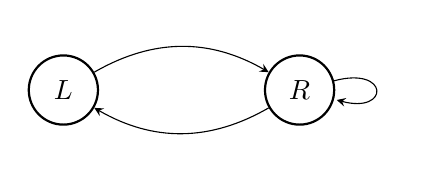
\begin{tikzpicture}[
    node distance=3cm,
    every state/.style={thick},
    ->,
    >=stealth
]

\node[state] (L) {$L$};
\node[state] (R) [right of=L] {$R$};

\draw (L) edge[bend left] node[above] {} (R);
\draw (R) edge[bend left] node[below] {} (L);
\draw (R) edge[loop right] node[right] {} (R);

\end{tikzpicture}

Note that the sting ``RRLLR'' is not allowed because `L' cannot transition to itself to make ``LL''.

Suppose that we have a matrix 
\[
A_{ij} = \begin{cases}
    1 \text{ if can transition from } L\to R\\
    0 \text{ else}
\end{cases}
\]
then we get a matrix of allowable transitions 
\[
A = \begin{bmatrix}
    0 & 1 \\ 1 & 1
\end{bmatrix}
\]

\subsection{Definition}

\underline{Definition of ``subshift of finite type''}: Let $\left\{R_1,\ldots, R_n\right\}$ be a Markov partition for $\Lambda$. Define 
\[
\Sigma_A = \left\{ a \in\left\{1,2,\ldots, n\right\}^{\mathbb{Z}} \text{ such that } A_{a_i\, a_{i+1}} \forall i \right\}
\]
Then $\sigma: \Sigma_A \to \Sigma_A$ is called a ``subshift of finite type'' with transition matrix $A$.

\subsection{Proposition 5.3.4}
\[
\begin{tikzcd}
\Lambda \arrow{r}{f} \arrow{d}{h} & \Lambda \arrow{d}{h} \\
\Sigma_A \arrow{r}{\sigma} & \Sigma_A
\end{tikzcd}
\]

\begin{mdframed}
    \subsection*{Intuition}
The big idea is that we are \textbf{encoding the dynamics of $f$ on $\Lambda$ using sequences of symbols}.

\subsubsection*{The Markov Partition}
The Markov partition $\{R_1, \ldots, R_n\}$ chops up the invariant set $\Lambda$ into $n$ regions. 
As you iterate a point $x \in \Lambda$ forward under $f$, it visits these regions in some order, 
producing a \textbf{bi-infinite sequence of symbols}:
\[
\ldots R_2, R_1, R_3, R_1, R_2, R_2, \ldots
\]
The map $h: \Lambda \to \Sigma_A$ is exactly this encoding --- it takes a point and returns the 
sequence of regions its orbit visits.

\subsubsection*{The Transition Matrix}
Not every sequence of symbols is dynamically realizable. The matrix $A$ encodes which transitions 
are \textbf{geometrically allowed} by the dynamics. In the period-3 example, $L \to L$ never happens 
because $f$ always maps $L$ outside of itself, so $A_{LL} = 0$.

\subsubsection*{The Commutative Diagram}
The diagram says that $h$ is a \textbf{conjugacy} between $f$ and $\sigma$, meaning:
\[
h \circ f = \sigma \circ h
\]
In words: iterating $f$ on $\Lambda$ and then encoding is the \textbf{same as} encoding first and 
then shifting the sequence left by one. This means:
\begin{itemize}
    \item The dynamics of $f$ on $\Lambda$ are \textbf{completely captured} by $\sigma$ on $\Sigma_A$
    \item $\sigma$ is just a left-shift on sequences, which is a much simpler object to study
    \item Any dynamical property of $\sigma$ (periodicity, chaos, entropy) \textbf{translates directly} 
    back to $f$
\end{itemize}

\subsubsection*{Why This is Powerful}
You have replaced a potentially complicated nonlinear map $f$ on a geometric set 
$\Lambda \subset \mathbb{R}^n$ with a simple \textbf{combinatorial shift map} on sequences of symbols. 
The complexity of the dynamics is now entirely captured by the combinatorics of the transition matrix $A$.
\end{mdframed}

\section{Smale-Birkhoff theorem}

Rowley sketched it, and it's so cool that I'm gonna just insert the photo:

\begin{figure}[h]
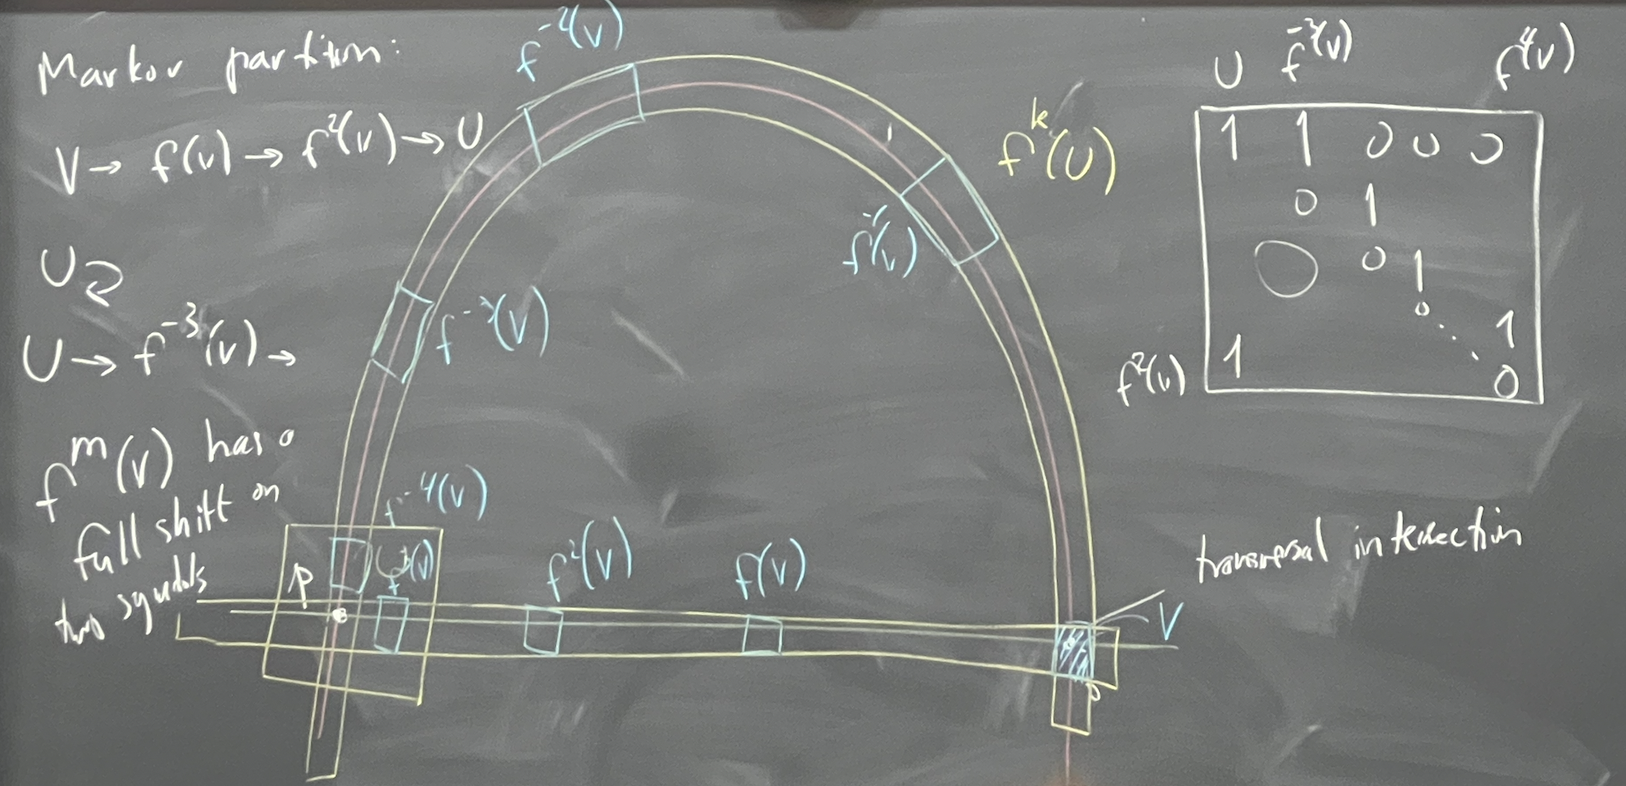
\includegraphics[width=\textwidth]{sketch_smale_birkhoff.png}
\end{figure}

The idea is to reason about the transition matrix $A$ about a Markov Partition of $f^m(V)\to U$. For a transversal intersection of the stable and unstable manifolds and some integer $m$, we have 
\[
A=\begin{bmatrix}
    1 & 1 \\ 1 & 1
\end{bmatrix}
\]
which is conjugate to the shift map, which implies dynamics that are sensitively dependent on initial conditions, and hence, chaos.

\begin{mdframed}
\subsubsection*{Things to tighten up}

\begin{enumerate}
    \item \textbf{What $f^m(V) \to U$ means.} The Markov partition is on the two rectangles 
    $\{U, V\}$ near $p$, not just on $f^m(V) \to U$. The all-ones matrix arises because all 
    transitions $U \to U$, $U \to V$, $V \to U$, and $V \to V$ are allowed.

    \item \textbf{Why $A$ has all ones.} The transversal homoclinic intersection, combined with 
    the Lambda lemma, is what forces $f^m(V)$ to stretch across \textbf{both} $U$ and $V$, 
    giving all entries equal to $1$. The all-ones structure does not come for free --- it is a 
    geometric consequence of the transversal intersection.

    \item \textbf{Conjugacy to the shift map.} One can be more precise: the dynamics on the 
    invariant set 
    \[
        \Lambda = \bigcap_{n\in\mathbb{Z}} f^n(U\cup V)
    \]
    are conjugate to the \textbf{full shift on two symbols} $\sigma: \Sigma_2 \to \Sigma_2$, 
    which gives sensitive dependence on initial conditions, a dense set of periodic orbits, 
    and the existence of a dense orbit.
\end{enumerate}
\end{mdframed}


\end{document}